\documentclass[letterpaper,10pt]{article}
\usepackage[utf8]{inputenc}
\usepackage[spanish,mexico]{babel}
\usepackage{amsmath}
\usepackage{amsfonts}
\usepackage{enumerate}
\usepackage{float}
\usepackage{indentfirst}
\usepackage{graphicx}
\usepackage{url}
\usepackage{multicol}
\usepackage{geometry}
\usepackage{fullpage}
\usepackage{hyperref}
\usepackage{tikz}
%\usetikzlibrary{shapes}
\usetikzlibrary{arrows,automata}

\tikzset{
    %Define standard arrow tip
    >=stealth',
    % Define arrow style
    pil/.style={
           ->,
           thick,}
}

\def\checkmark{\tikz\fill[scale=0.4](0,.35) -- (.25,0) -- (1,.7) -- (.25,.15) -- cycle;}

\begin{document}

\thispagestyle{empty}
 	
\begin{minipage}[t]{0.6\textwidth}

{\LARGE \textbf{INF152} Estructuras Discretas}

{\large Profesores: Margarita Bugueño, Sebastián Gallardo.}\\
{\large Ayudantes: Valentina Aróstica, Bryan González, Sofía Mañana y Sofía Riquelme}

Universidad T\'ecnica Federico Santa Mar\'{\i}a

Departamento de Inform\'atica -- CSJ - CC 

Noviembre 8, 2021

\end{minipage}
\hfill
\begin{minipage}[t]{0.3\textwidth}
Nombre:

\begin{tabular}{|c|}\hline
%%%%%%%%%%%%%%%%%%%%%%%% !!!! LEER !!!!  %%%%%%%%%%%%%%%%%%%%%%%%%%%%%%
% Borre los caracteres ~ y los signo peso $, para poner su nombre aquí: %
Diego Eduardo Paz Letelier\\\hline
\end{tabular}

\vspace{0.1cm}

Rol:

\begin{tabular}{|c|c|c|c|c|c|c|c|c|c|c|}\hline
%%%%%%%%%%%%%%%%%%%%%%%% !!!! LEER !!!!  %%%%%%%%%%%%%%%%%%%%%%%%%%%%%%
% NO borre los caracteres ampersand &, entre ellos ponga cada dígito de su rol:%
%EJEMPLO: 2 & 0 & 2 & 0 & 7 & 3 & 5 & 0 & 0 & 0
2 & 0 & 2 & 0 & 0 & 4 & 5 & 0 & 2 & - & K\\\hline
\end{tabular}
\end{minipage}

\vspace{0.3cm}

\begin{center}
    \huge Tarea 2
\end{center}

\section{Reglas generales}
\begin{itemize}
    \item Esta tarea tiene como objetivo, el que usted aprenda a usar \LaTeX, y que refresque los contenidos relacionados con el Certamen 2. 
    \item Debe investigar por su cuenta la sintáxis de \LaTeX $~$para adquirir las herramientas que le permitan elaborar un desarrollo claro, ordenado, y \textbf{formal} en cada pregunta.
    
    \item Para resolver cada pregunta, debe hacer uso de los contenidos, algoritmos y métodos aprendidos en el curso (Demostración, Isomorfismo, Teoremas, Tablas de adyacencia, Grafos, Búsqueda en Profundidad y a lo Ancho, etc). Si su respuesta final es correcta, pero se ha utilizado un método distinto al enseñado en clases no se asignará puntaje. Ídem si entrega resultados sin desarrollo. 
    
    \item No se permite adjuntar/incluir fotografías de grafos o tablas en este archivo. Ya sean dibujadas a mano, en word, en herramientas virtuales de dibujo, etc. Si los grafos y tablas no están hechas en \LaTeX no obtendrá puntaje. 
    
    \item La tarea debe realizarse de manera individual. Cabe decir, que el buscar por su cuenta la solución a los problemas aquí planteados, y aprender a usar \LaTeX  $~$mientras desarrolla, le será de mucha utilidad tanto en este curso, como en otros futuros.
    
    \item Debe entregar una carpeta comprimida en .zip que contenga el (o los) archivo(s) .tex con sus respuestas, y las imágenes que van incluidas en el proyecto. El nombre del .zip debe ser su nombre y apellido. Ejemplo:\\ Nombre\_Apellido.zip. En este caso no es necesario agregar el PDF, dado que se compilará cada proyecto a la hora de revisar.
    
    \item Para compilar el proyecto al revisar, se usará el editor de texto Overleaf.
    
    \item Revise 2 veces que el proyecto (zip) que vaya a entregar sea correcto y que contenga todas sus respuestas. Se revisará sólo lo entregado sin opción de hacer una segunda entrega.
    
    \item Tiene hasta las 23:59 hrs del día 17 de Noviembre para entregar esta tarea vía Aula.
    
    \item Se descontarán 10 puntos por atraso desde las 00:01 hrs hasta las 01:00 hrs, y se irán restando sucesivamente 10 puntos de su nota por cada hora de atraso.
    
    \item \textbf{Se descontarán 5 puntos por cada warning.} Su archivo .tex \textbf{DEBE} compilar. (se descontará 100 puntos si no lo hace). Errores y warnings no son lo mismo. Si su código tiene errores probablemente su .tex no compile, aunque es posible que algunos editores de \LaTeX $~$generen un PDF de todas formas. Procure corregir todos los errores y warnings antes de entregar.
    
    
\end{itemize}


\section{Isomorfismo}
\begin{enumerate}
    \item Debido a que la USM esta en proceso de volver a sus andanzas presenciales, los ayudantes de Estructuras Discretas fueron los elegidos para realizar un mapa a través de las dependencias de la Universidad. La tarea que fue encomendada es la creación de un Grafo que represente las conecciones directas que tiene cada sala entre sí, en un edificio de la USM. Los ayudantes consiguieron hacer una tabla de adyacencia con las conecciones directas entre las salas, cada una nombrada con las letras de la O a la X, pero el estrés de la sobrecarga académica los dejó inhabilitados para dibujar el grafo; ahí es donde entran ustedes, los estudiantes de Estructuras Discretas. Considerando la siguiente tabla de adyacencia (que les dejaron sus queridos ayudantes), utilice las herramientas que \LaTeX \:ofrece para dibujar con el paquete tikz el Grafo \ref{tab:G1} (10\%).

        \begin{table}[H]
        \centering
        \begin{tabular}{c|cccccccccc}
               & O & P & Q & R & S & T & U & V & W & X \\
             \hline
             O & 0 & 1 & 0 & 0 & 0 & 0 & 0 & 0 & 1 & 1\\
             P &   & 0 & 1 & 0 & 0 & 1 & 0 & 0 & 0 & 0\\
             Q &   &   & 0 & 1 & 0 & 0 & 0 & 1 & 0 & 0\\
             R &   &   &   & 0 & 0 & 0 & 0 & 0 & 0 & 1\\
             S &   &   &   &   & 0 & 1 & 0 & 0 & 1 & 0\\
             T &   &   &   &   &   & 0 & 1 & 0 & 0 & 0\\
             U &   &   &   &   &   &   & 0 & 1 & 0 & 1\\
             V &   &   &   &   &   &   &   & 0 & 1 & 0\\
             W &   &   &   &   &   &   &   &   & 0 & 0\\
             X &   &   &   &   &   &   &   &   &   & 0\\
        \end{tabular} 
        \caption{Tabla de Adyacencia Grafo 1}
        \label{tab:G1}
    \end{table}
    
%%%%%%%%%%%%%%%%%%%%%%%%%%%%%%%%%%%%%%%%%%%%%%%%%%%%%%%%%%%%%%%%%%%%%%%%%%%%%%%%%%%%%%%%%%%%%%%%%%%%%%%%%%%%%%%%%%%%%%%%%%%%%%%%%%%%%%%%%%%%%%%%%%%%%%%%%%%%%%%%%%%%%%%%%%%%%%%%%%%%%%%%%%%%%%%%%%%%%%%%%%%%%%%%%%%%%
\textbf{Solución:}
%Escriba su respuesta aquí
\begin{center}
    \begin{minipage}{0.9\textwidth}
    \centering
        \begin{tikzpicture}[scale=1,transform shape,node distance=1.7cm,main node/.style={circle,draw}]
                        \node[main node] (1)  {$O$};
                        \node[main node] (2) [above of=1] {$P$};
                        \node[main node] (3) [above right of=2]  {$Q$};
                        \node[main node] (4) [right of=3]  {$R$};
                        \node[main node] (5) [below right of=1] {$X$};
                        \node[main node] (6) [right of=5] {$W$};
                        \node[main node] (7) [right of=6] {$V$};
                        \node[main node] (8) [above right of=7] {$U$};
                        \node[main node] (9) [above of=8] {$T$};
                        \node[main node] (10) [above left of=9] {$S$};

                        %\path (1) edge [bend left,-] (2);
                        \draw[] (1)--(2);
                        \draw[] (2)--(3);
                        \draw[] (3)--(4);
                        \draw[] (1)--(6);
                        \draw[] (5)--(1);
                        \draw[] (5)--(4);
                        \draw[] (6)--(10);
                        \draw[] (9)--(10);
                        \draw[] (8)--(9);
                        \draw[] (7)--(6);
                        \draw[] (8)--(7);
                        \draw[] (5)--(8);
                        \draw[] (3)--(7);
        \end{tikzpicture}
    \label{sol1}
    \end{minipage}
\end{center}

    
    \item Otro grupo de ayudantes se adelantó, y construyeron su propio grafo con conexiones. Ahora la Universidad necesita saber si ambos grafos son válidos, por lo que se les pide que demuestren o refuten que el Grafo \ref{tab:G1} y el Grafo 2 (que se muestra a continuación) son (o no) isomorfos. Argumente formalmente y escriba una conclusión. (30\%)
    \begin{center}
    %Esta imagen está adjunta en lugar de dibujada con latex, porque queremos que se esfuercen por dibujar el grafo G1 ustedes mismos, y que no "copien" el código de G2.
    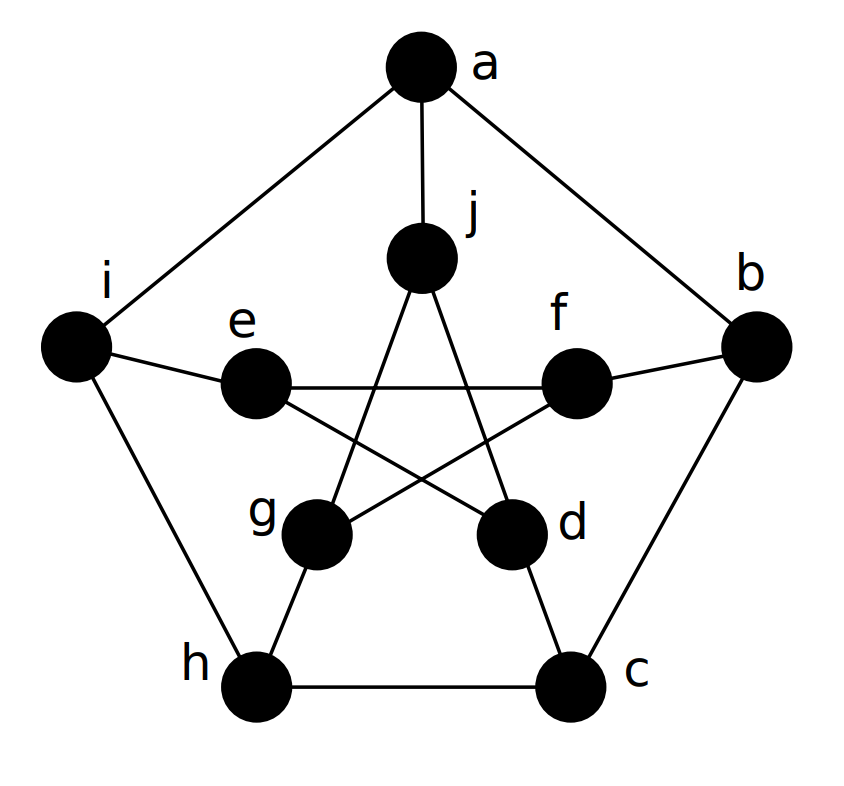
\includegraphics[scale=0.25]{Screenshot_3.png}\\
    Figura 1: Grafo 2
    \end{center} 
    
%%%%%%%%%%%%%%%%%%%%%%%%%%%%%%%%%%%%%%%%%%%%%%%%%%%%%%%%%%%%%%%%%%%%%%%%%%%%%%%%%%%%%%%%%%%%%%%%%%%%%%%%%%%%%%%%%%%%%%%%%%%%%%%%%%%%%%%%%%%%%%%%%%%%%%%%%%%%%%%%%%%%%%%%%%%%%%%%%%%%%%%%%%%%%%%%%%%%%%%%%%%%%%%%%%%%%
    
\textbf{Solución:}
%Escriba su respuesta aquí

\end{enumerate}
\newpage
\section{Búsqueda}
\begin{enumerate}
    \item El pasado fin de semana largo, un grupo de amigos aprovechó que tenían algunos de los días libres, entre tanto estudio, para ir a distraerse y se propusieron ir durante un día completo al parque de diversiones \textit{``Sansanolandia''}. Para ello, quedaron de juntarse en el \textit{Parque Santa María} que queda muy cerca. Dos entusiastas amigos del grupo están cursando el ramo \textit{Estructuras Discretas} y decidieron representar el parque en el grafo de la Tabla \ref{tab:parque}. Además, para abreviar, numeraron los vértices de acuerdo a la información de la Tabla \ref{tab:atracciones}. 
    
    \begin{minipage}[h]{0.36\textwidth}
    \small
    \begin{table}[H]
        \begin{center}
            
            \begin{tabular}{c|cccccccccc}
            
             & $a_1$ & $a_2$ & $a_3$ & $a_4$ & $a_5$ & $a_6$ & $a_7$ & $a_8$ & $a_9$ & $a_{10}$\\ \hline
            $a_1$ & 0 & 1 & 0 & 0 & 0 & 1 & 0 & 0 & 0 & 0\\
            $a_2$ & 1 & 0 & 0 & 0 & 1 & 1 & 1 & 0 & 0 & 0\\
            $a_3$ & 0 & 0 & 0 & 0 & 0 & 0 & 0 & 0 & 0 & 1\\
            $a_4$ & 0 & 0 & 0 & 0 & 1 & 0 & 1 & 0 & 0 & 0\\
            $a_5$ & 0 & 1 & 0 & 1 & 0 & 0 & 0 & 0 & 0 & 0\\
            $a_6$ & 1 & 1 & 0 & 0 & 0 & 0 & 1 & 0 & 1 & 1\\
            $a_7$ & 0 & 1 & 0 & 1 & 0 & 1 & 0 & 0 & 0 & 0\\
            $a_8$ & 0 & 0 & 0 & 0 & 0 & 0 & 0 & 0 & 1 & 1\\
            $a_9$ & 0 & 0 & 0 & 0 & 0 & 1 & 0 & 1 & 0 & 0\\
            $a_{10}$ & 0 & 0 & 1 & 0 & 0 & 1 & 0 & 1 & 0 & 0\\
            \end{tabular}
        \caption{Representación del parque.}\label{tab:parque}
        
        \end{center}
    \end{table}
    
    \end{minipage}
    \hfill
    \begin{minipage}[h]{0.40\textwidth}
    \footnotesize
    \begin{table}[H]
        \begin{center}
            
            \begin{tabular}{|c|l|}
            \hline
            \textbf{Vértice} & \textbf{Lugar}\\ \hline
            $a_1$ & Sansanolution\\
            $a_2$ & Autitos Sansanos Chocones\\
            $a_3$ & Sansano Rawr\\
            $a_4$ & Boletería\\
            $a_5$ & Las Hojas de Sethi\\
            $a_6$ & Coloreo Matching\\
            $a_7$ & Tazas EGF\\
            $a_8$ & Casa Fantasmal Hamiltoniana\\
            $a_9$ & Tagasansanoda\\
            $a_{10}$ & Montaña Sansana\\
            \hline
            \end{tabular}
        \caption{Lugares del parque.}\label{tab:atracciones}
        \end{center}
    \end{table}
    \end{minipage}
    \begin{itemize}
        \item[a) ]Dibuje, utilizando las herramientas que ofrece \LaTeX  $~$el grafo correspondiente. (10\%)
        
        \textbf{Solución:}
        %Escriba su respuesta aquí
        \begin{center}
            \begin{minipage}{0.9\textwidth}
            \centering
                \begin{tikzpicture}[scale=1,transform shape,node distance=2cm,main node/.style={circle,draw}]
                        \node[main node] (1){$a_{1}$};
                        \node[main node] [above of=1] (2){$a_{2}$};
                        \node[main node] [right of=10] (3){$a_{3}$};
                        \node[main node] [above left of=7] (4){$a_{4}$};
                        \node[main node] [above right of=2] (5){$a_{5}$};
                        \node[main node] [below right of=1] (6){$a_{6}$};
                        \node[main node] [right of=6] (7){$a_{7}$};
                        \node[main node] [below right of=10] (8){$a_{8}$};
                        \node[main node] [above right of =7] (9){$a_{9}$};
                        \node[main node] [right of=5] (10){$a_{10}$};

                        \draw[] (1)--(2);
                        \draw[] (1)--(6);
                        \draw[] (2)--(5);
                        \draw[] (2)--(6);
                        \draw[] (2)--(7);
                        \draw[] (3)--(10);
                        \draw[] (4)--(5);
                        \draw[] (4)--(7);
                        \draw[] (6)--(7);
                        \draw[] (6)--(9);
                        \draw[] (6)--(10);
                        \draw[] (8)--(9);
                        \draw[] (8)--(10);


                \end{tikzpicture}
                \label{sol3}
                \end{minipage}
            \end{center}
            
        \item[b) ]El grupo desea llegar lo más pronto posible a la atracción \textit{Sansano Rawr} desde la boletería. ¿Es más eficiente utilizar, búsqueda a lo ancho o en profundidad? Justifique, mostrando paso a paso cómo realiza cada búsqueda, y mostrando el orden en que se visitan los lugares en casa caso. (50\%)
        
        \textbf{Solución:}
        %Escriba su respuesta aquí
        \newline
        tuve toda la semana llena y no tuve tiempo pa hacer la tarea :(
        
    \end{itemize}


\end{enumerate}


\newpage

\section*{Hint}

El package Tikz de \LaTeX $~$ permite hacer imágenes a partir código como se aprecia en la figura:

\begin{center}
    \begin{minipage}{0.32\textwidth}
    \centering
        \begin{tikzpicture}[scale=1,transform shape,node distance=2.2cm,main node/.style={circle,draw}]
        		%nodes
        			  \node[main node,label={P}, very thick] (1) 			{$X$};
        			  \node[main node] (2) [above right of=1] 	{$Z$};
        		%Edges
        			  \path (1) edge [bend left,-]  (2);
        \end{tikzpicture}
    \label{gra2}
    \end{minipage}
\end{center}



\end{document}
